\section{Iteración VIII}
\subsection{Resumen}
Aquí desarrollamos una plataforma web para que los usuarios registrados puedan gestionar sus propias categorías de muebles y subir sus muebles para poder usarlos dentro de la aplicación.

\subsection{Desarrollo}
La plataforma cuenta también con un login para acceder a la cuenta que el usuario creó desde la aplicación (ver figura 4.57).

\begin{figure}[hbt!]
	\centering
	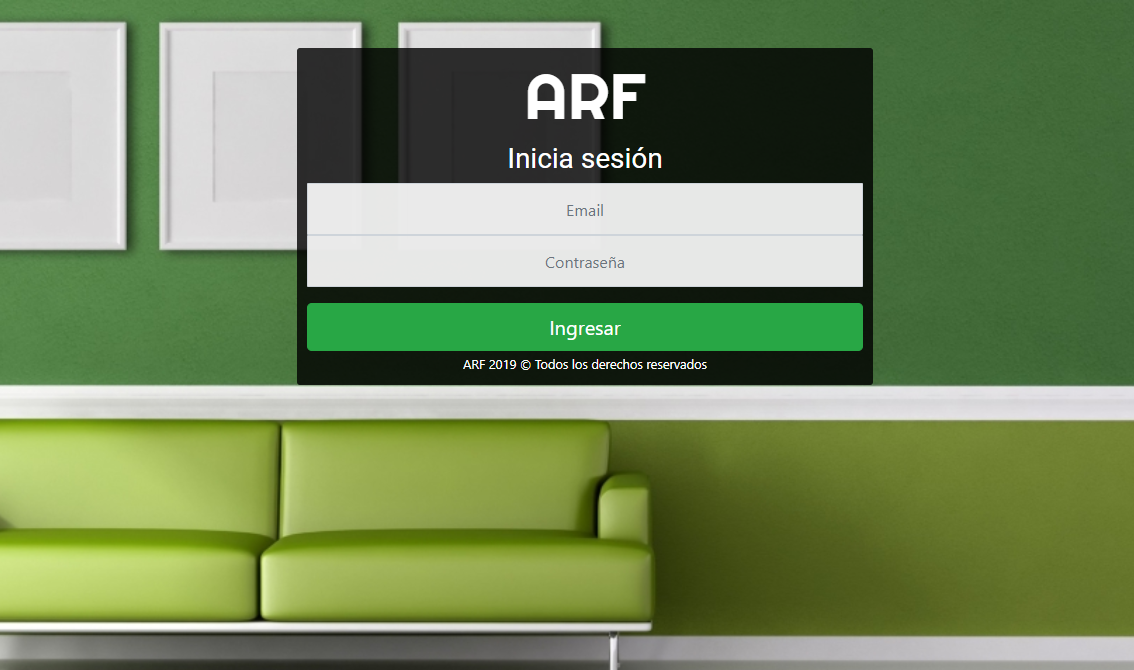
\includegraphics[width=15cm,height=9cm]{imagenes/desarrollo/app/WEB_LOGIN.png}
	\caption{Login de aplicación web.}
	\label{fig:weblogin}
\end{figure}

Tras iniciar sesión, se muestra un dashboard con todos los muebles que ha subido (ver figura 4.58) y visualizarlos en 3D (ver figura 4.59).

\begin{figure}[hbt!]
	\centering
	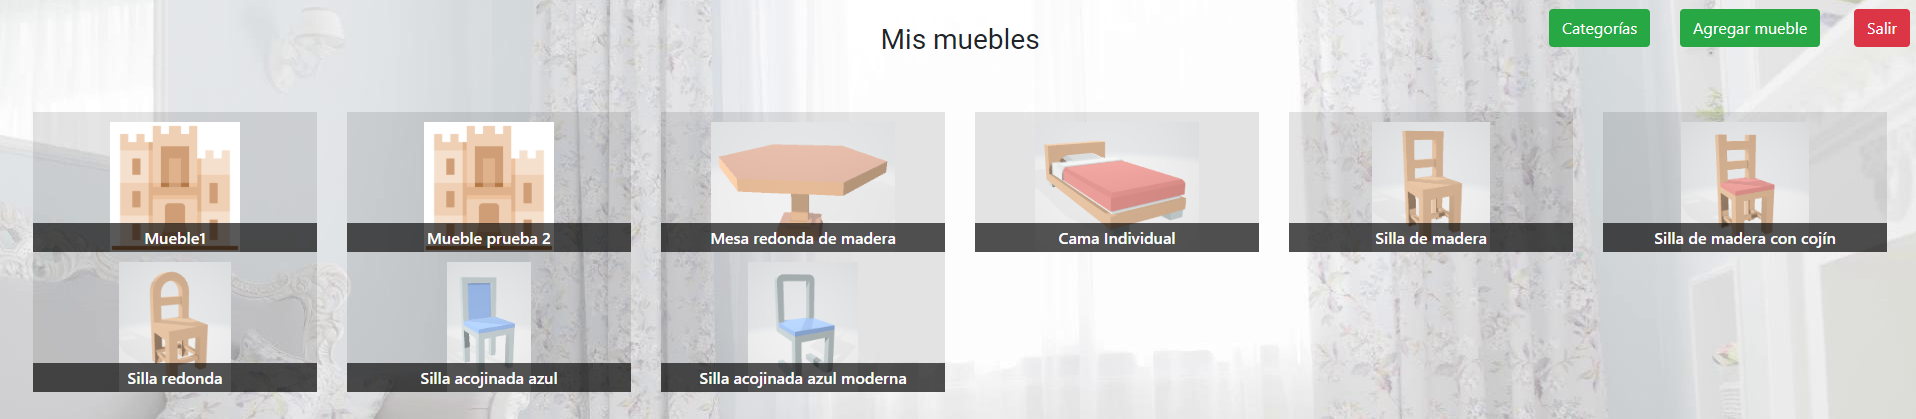
\includegraphics[width=17cm,height=4cm]{imagenes/desarrollo/app/WEB_FURNITURES.png}
	\caption{Lista de muebles del usuario.}
	\label{fig:weblogin}
\end{figure}
\begin{figure}[hbt!]
	\centering
	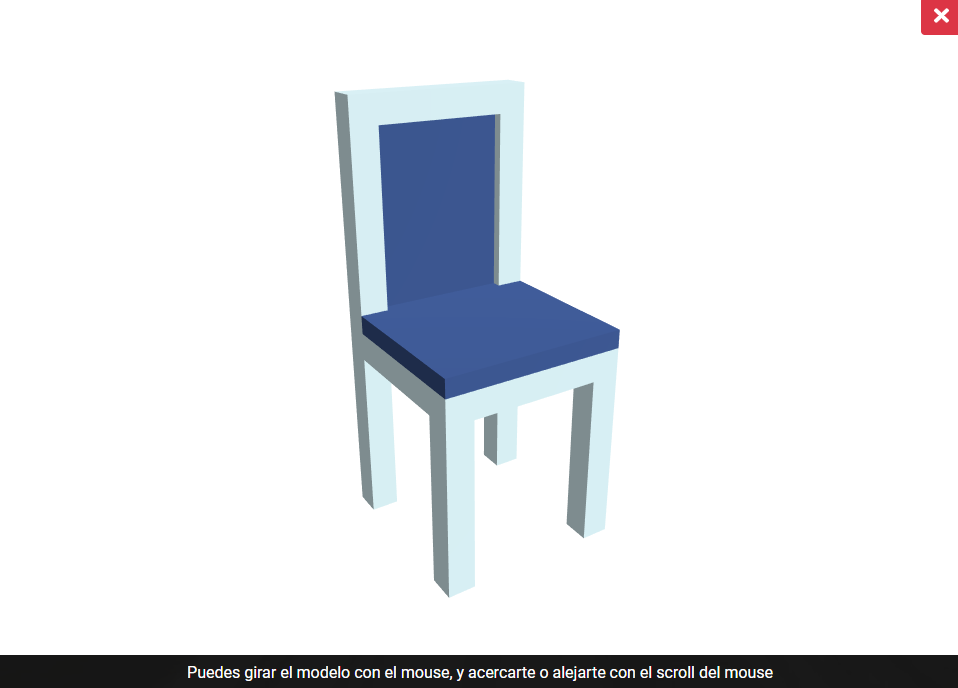
\includegraphics[width=15cm,height=9cm]{imagenes/desarrollo/app/WEB_MODEL.png}
	\caption{Visor de muebles.}
	\label{fig:webviewer}
\end{figure}

Desde aquí el usuario puede agregar, crear, modificar y eliminar categorías y subcategorías (ver figura 4.60) y agregar muebles (ver figura 4.61). Para agregar un mueble se requiere lo siguiente
\begin{itemize}
	\item Nombre del mueble
	\item Precio
	\item Categoría
	\item Subcategoría
	\item Un ZIP con los recursos del modelo en 3D.
	\item Una imagen del  mueble
\end{itemize}
Del proceso anterior hay dos elementos de suma importancia:\par
\textbf{ZIP de modelo}.- En la raíz de este ZIP deben estar todos los archivos del modelo en \textbf{formato glTF}, formato necesario para poder recuperar el mueble de la nube y usarlo en la realidad aumentada en tiempo de ejecución. \par
\textbf{Imagen del mueble}.- Es una imagen que identifique al mueble. Esta imagen se mostará en el menú de muebles al crear un escenario.\par



\begin{figure}[hbt!]
	\centering
	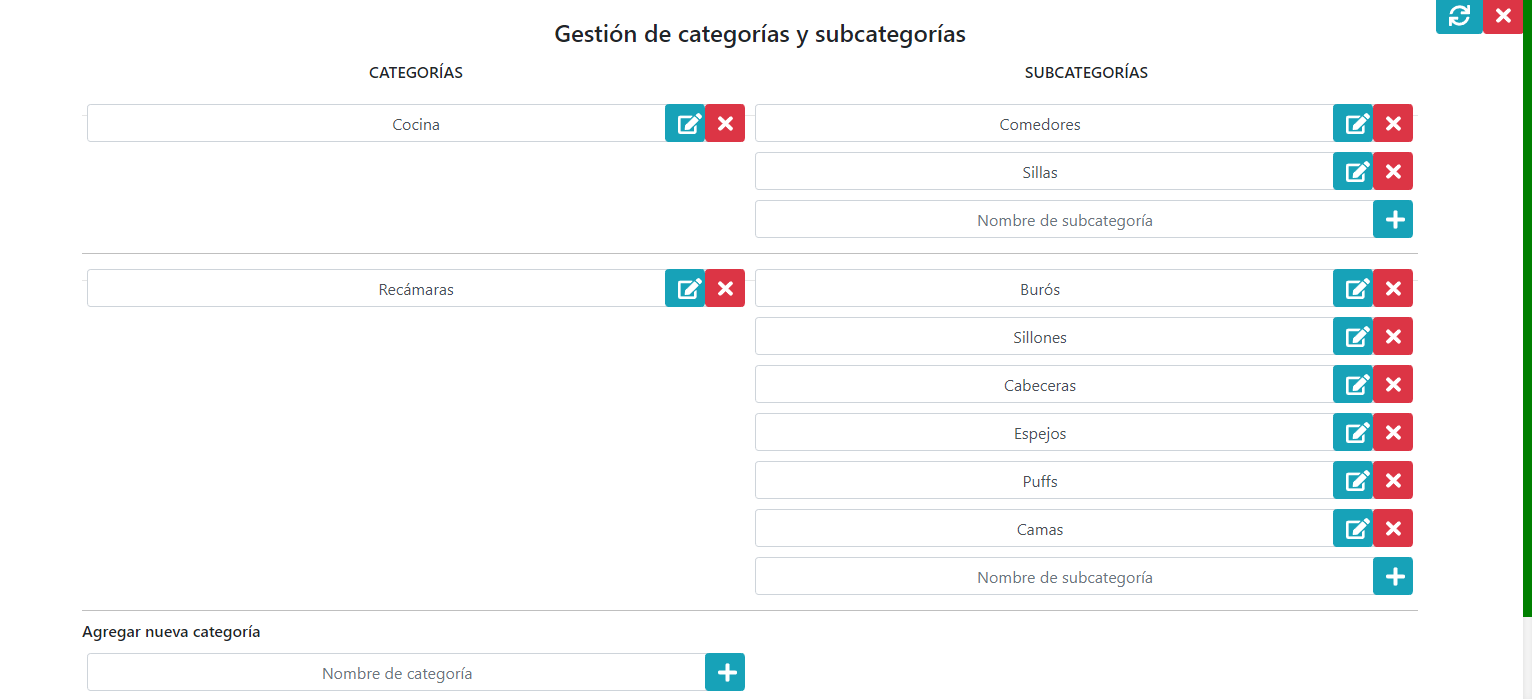
\includegraphics[width=15cm,height=7cm]{imagenes/desarrollo/app/WEB_CATEGORIES.png}
	\caption{Gestión de categorías y subcategorías.}
	\label{fig:webcat}
\end{figure}
\begin{figure}[hbt!]
	\centering
	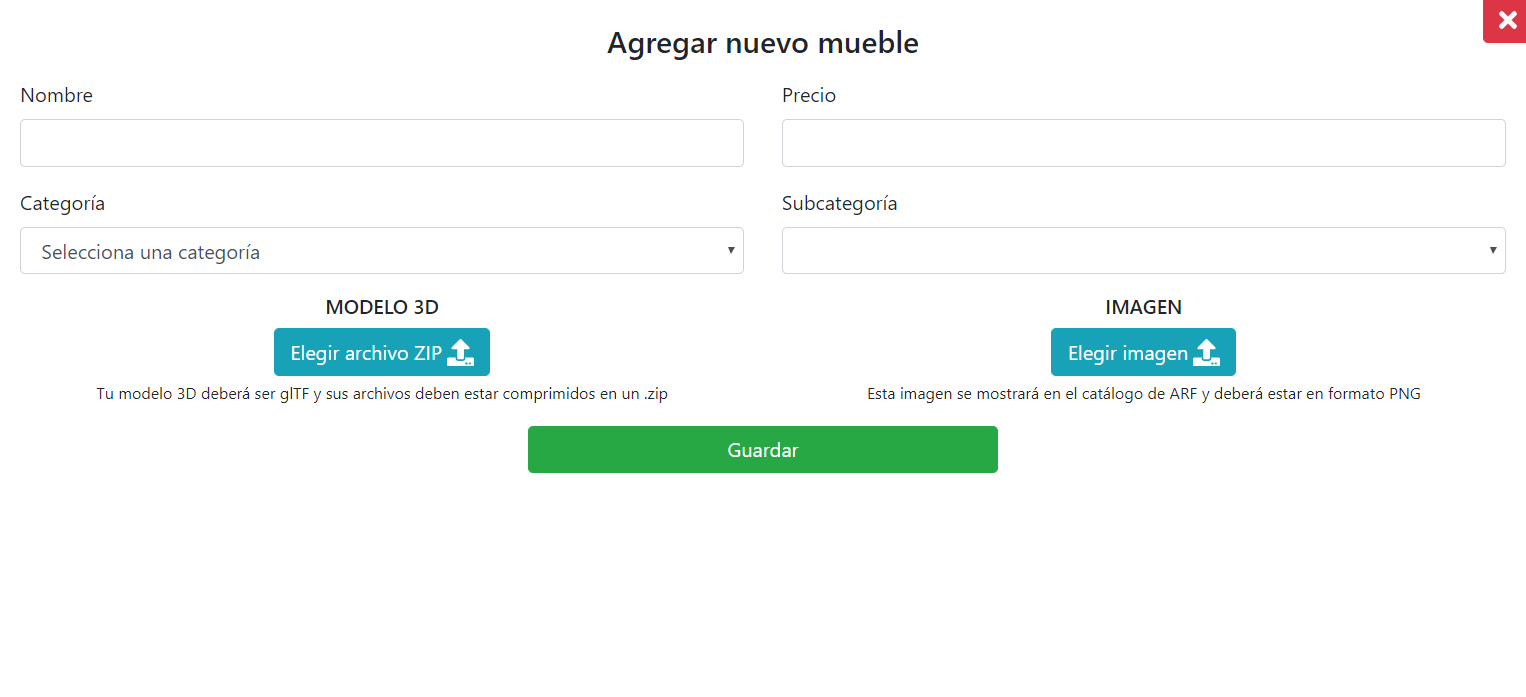
\includegraphics[width=15cm,height=7cm]{imagenes/desarrollo/app/WEB_ADD.png}
	\caption{Módulo para agregar muebles.}
	\label{fig:webadd}
\end{figure}

Esta funcionalidad cumple con un proceso de negocio general para la subida de muebles a la plataforma web (ver figura 4.62)

\begin{figure}[h!]
	\centering
	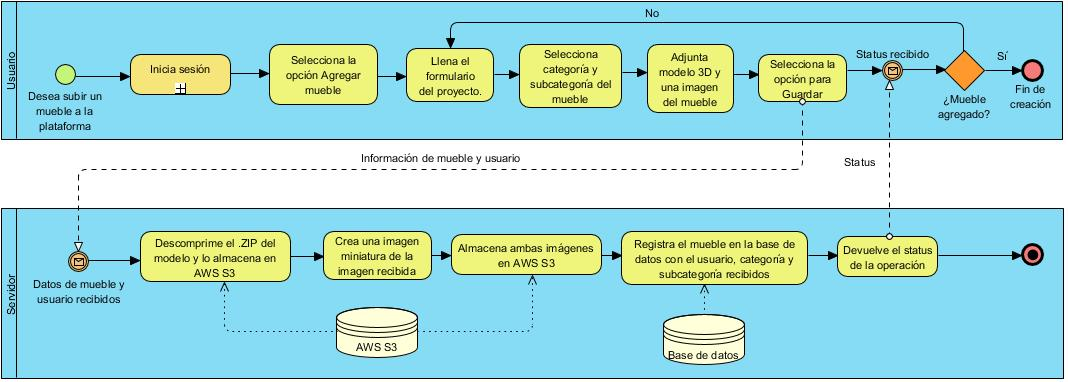
\includegraphics[width=15cm,height=6cm]{imagenes/desarrollo/diagramas/BPMN_UPLOAD_FURNITURE.jpg}
	\caption{Diagrama de proceso de subida de muebles.}
	\label{fig:recover}
\end{figure}
\clearpage